%!TEX program = xelatex
%%%%%%%%%%%%%%%%%%%%%%%这是导言部分的开始%%%%%%%%

%========= 导言部分声明文档的类型=================
\documentclass{article}

%=========导言部分可可以加载宏包=================
\usepackage{amsmath}                % 数学公式排版宏包
\usepackage{amssymb}                % 数学符号命令宏包
\usepackage{amsthm}                 % 数学定理宏包
\usepackage[UTF8]{ctex}             % 中文输入宏包
\usepackage[a4paper]{geometry}      % 页面设置宏包
\usepackage{setspace}               % 行间距宏包
\usepackage{graphicx}               % 图片宏包
\usepackage{listings}               % 代码宏包
\usepackage{color}					% 颜色宏包
\usepackage{xcolor}                 % 颜色处理宏包
\usepackage{float}                  % 浮动对象式样宏包
\usepackage{fontspec}
\usepackage{enumerate}				% 列举编号包

%=========页面设置==============================
\geometry{left=1cm,right=1cm,top=1cm,bottom=2cm}
\onehalfspacing
\setlength\parindent{0em}

%=========代码格式设置============================
\definecolor{dkgreen}{rgb}{0,0.6,0}
\definecolor{gray}{rgb}{0.5,0.5,0.5}
\definecolor{mauve}{rgb}{0.58,0,0.82}
% \setmonofont{Consolas}
\lstset{
	numbers = left, 	
	numberstyle = \color{gray}, 
	keywordstyle = \color{blue},
	commentstyle = \color{dkgreen}, 
	stringstyle = \color{mauve},
	basicstyle = \ttfamily,
	breaklines = true,
	frame = shadowbox, % 阴影效果
	rulesepcolor = \color{ red!20!green!20!blue!20} ,
	escapeinside = ``, % 英文分号中可写入中文
	xleftmargin = 2em,xrightmargin=2em, aboveskip=1em,
	framexleftmargin = 2em
} 

%=========导言部分可以定义标题信息===============
\title{组会报告}
\author{徐益}
\date{\today}
%%%%%%%%%%%%%%%%%%%%%%%这是导言部分的结束%%%%%%%%%

%%%%%%%%%%%%%%%%%%%%%%%这是正文部分的开始%%%%%%%%%
\begin{document}

%=========生成标题================================
\maketitle

%=========开始正文的输入==========================

%===========第一节=================
\section{工作内容} 
1. 设计可复用的MAC-PHY连调结构;

2. 实现MAC-PHY连调结构PHY层部分线程并测试。

3. 协助MAC层目录结构搭建。

%===========第二节=================
\section{设计可复用的MAC-PHY连调结构}
\subsection{结构}
\begin{figure}[H]
	\centering
	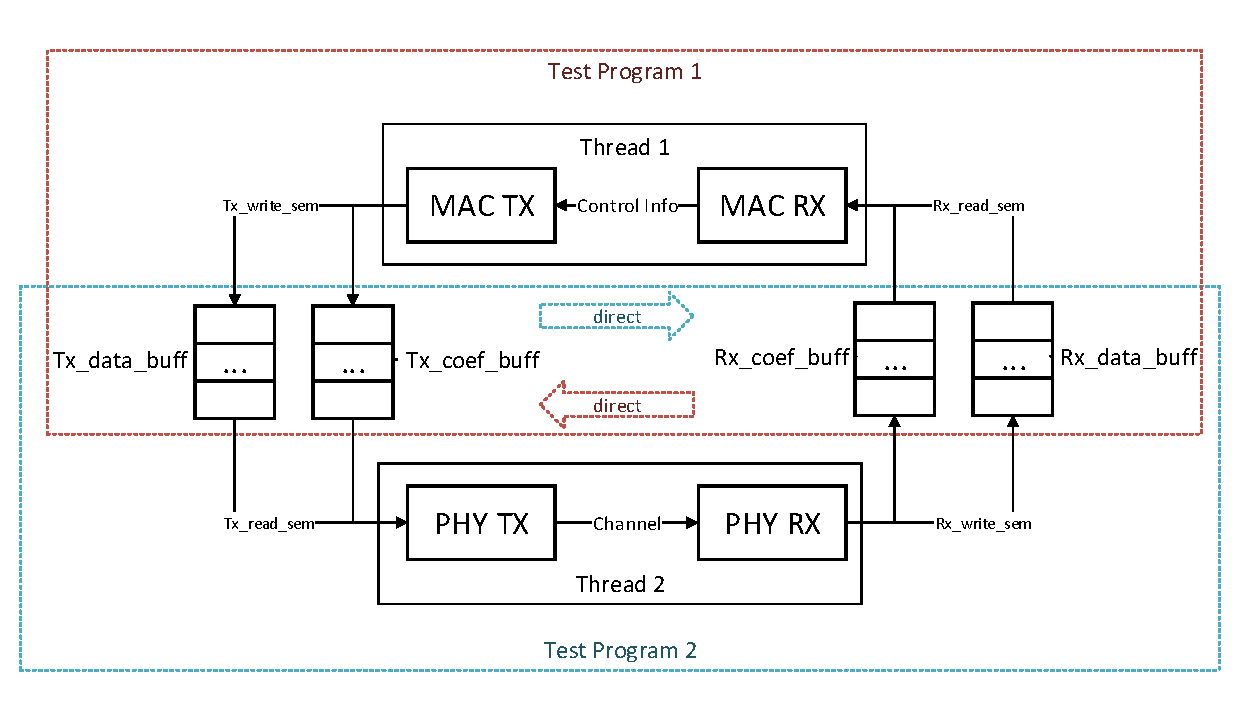
\includegraphics[width = \textwidth]{structure.pdf}
	\caption{MAC-PHY连调结构}
\end{figure}
\subsection{优势}
1. 各Buffer级信号量指针通过线程参数传递,避免全局变量的使用;\\
2. 各线程可进行独立测试调试;\\
3. 各线程封装度高,易于维护替换。


%===========第三节=================
\section{实现MAC-PHY连调结构PHY层部分线程}
\subsection{PHY线程参数}
\lstset{language=C++}
\begin{lstlisting}
typedef struct nr5g_phy_tx_rx_sgl_thrd_t
{
    float snr;                          // 测试信噪比
    int32_t max_len_flag;               // 是否使用最大传输长度
    int32_t max_tb_byte_len;            // 每个TB的最大长度(Byte)

    int8_t **tx_data_buff;              // Tx数据Buffer
    nr5g_phy_tx_coef_t *tx_coef_buff;   // Tx参数Buffer
    int32_t tx_buff_size;               // Tx中Buffer长度

    int8_t **rx_data_buff;              // Rx数据Buffer
    nr5g_phy_rx_coef_t *rx_coef_buff;   // Rx参数Buffer
    int32_t rx_buff_size;               // Rx中Buffer长度

    sem_t* tx_read_sem;                 // Tx读信号量
    sem_t* tx_write_sem;                // Tx写信号量
    sem_t* rx_read_sem;                 // Rx读信号量
    sem_t* rx_write_sem;                // Rx写信号量
    sem_t* destroy_sem;                 // 线程销毁信号量

} nr5g_phy_tx_rx_sgl_thrd_t;

\end{lstlisting}

\subsection{Tx Buffer 参数}
\lstset{language=C++}
\begin{lstlisting}
typedef struct nr5g_phy_tx_coef_t
{
    int32_t subframe_indx;                  // 子帧号
    int32_t cqi_list[MAX_TB_NUM];           // CQI列表
    int32_t max_layer_num_list[MAX_TB_NUM]; // 最大流数列表
    int32_t tb_byte_len_list[MAX_TB_NUM];   // TB长度列表

} nr5g_phy_tx_coef_t;

\end{lstlisting}

\subsection{Rx Buffer 参数}
\lstset{language=C++}
\begin{lstlisting}
typedef struct nr5g_phy_rx_coef_t
{
    int32_t crc_result_buff[MAX_TB_NUM];    // CRC校验结果

} nr5g_phy_rx_coef_t;

\end{lstlisting}

%===========第四节=================
\section{目录结构}
\begin{figure}[H]
	\centering
	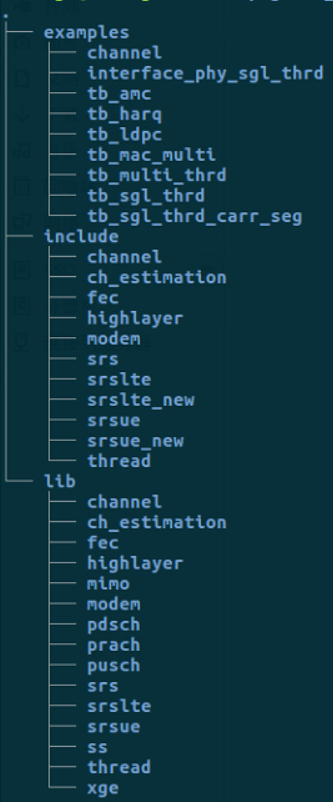
\includegraphics[width = .4\textwidth]{5gmimo.png}
	\caption{5gmimo目录结构}
\end{figure}

%===========第五节=================
% \section{有PRACH情况下的资源分配问题}
% \begin{figure}[H]
% 	\centering
% 	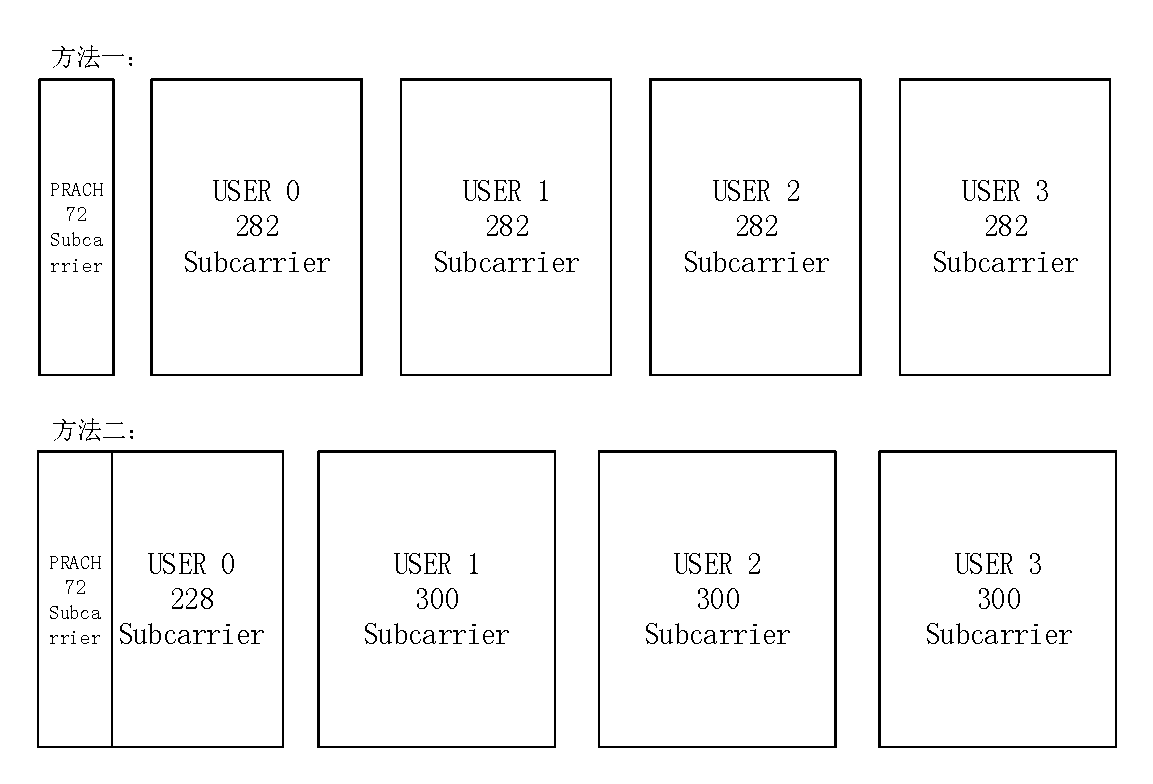
\includegraphics[width = \textwidth]{ques.pdf}
% 	\caption{两种方案}
% \end{figure}

%===========下周计划=================
% \section{下阶段计划}
% 1. 完善单线程系统(修复Bug)

\end{document}
%%%%%%%%%%%%%%%%%%%%%%%这是正文部分的结束%%%%%%%%%%%%